
%%%%%%%%%%%%%%%%%%%% file CSMC_MUME_LaTeX_Template.tex %%%%%%%%%%%%%%%%%%%%%
%
% This is the LaTeX source for the instructions to authors using
% the LaTeX document class 'llncs.cls' for contributions to
% the Journal of Creative Music Systems.
% Copyright: http://www.springer.com/lncs       Springer Heidelberg 2006/05/04
%
% It may be used as a template for your own input - copy it
% to a new file with a new name and use it as the basis
% for your article.
%
% NB: the document class 'llncs' has its own and detailed documentation, see
% ftp://ftp.springer.de/data/pubftp/pub/tex/latex/llncs/latex2e/llncsdoc.pdf
%
%%%%%%%%%%%%%%%%%%%%%%%%%%%%%%%%%%%%%%%%%%%%%%%%%%%%%%%%%%%%%%%%%%%

\documentclass[runningheads,a4paper]{llncs}

\usepackage{amssymb}
\setcounter{tocdepth}{3}
\usepackage{graphicx}
\usepackage{url}
\usepackage{apacite}
%added 
\usepackage[inline]{enumitem}    
\usepackage{subcaption}
\usepackage{caption}
\usepackage{threeparttable} %annotations for table
\usepackage{csquotes}
\usepackage{appendix}

\newcommand{\keywords}[1]{\par\addvspace\baselineskip
\noindent\keywordname\enspace\ignorespaces#1}

\pagestyle{headings}

\begin{document}

\mainmatter  

\title{Percussive Sound Generation with Virtual Listeners and Modular Synthesizers}

% a short form should be given in case it is too long for the running head
\titlerunning{Virtual Percussive Sound Generation}

% the name(s) of the author(s) follow(s) next
\author{Amir Salimi \and Abram Hindle}

\authorrunning{Amir Salimi and Abram Hindle }

% the affiliations are given next; don't give your e-mail address
% unless you accept that it will be published
\institute{Department of Computing Science\\ University of Alberta \\ \email{asalimi@ualberta.ca}}

% intro, 1 page
% background and methodology 2 pages
% implementation 
% results 2.5
\maketitle

\begin{abstract}
Digital sound artists often require a variety of percussive samples for their music. For more than two decades research involving digital synthesis, heuristic search, and neural networks has been used for the generation of novel sounds. This work is a proof of concept in automatic programming of synthesizers towards their best approximation of drum sounds. We centered our approach around the combination of two central components: \begin {enumerate*} [label=(\roman*)] \item a \emph{virtual ear} capable of evaluating the proximity of \enquote{unusual} sounds to drum sounds and \item a dynamic \emph{virtual synthesizer} with a rich set of tractable parameters\end{enumerate*}. We present a generative pipeline that utilizes classical digital signal processing functions guided by supervised learning towards the generation of one-shot percussive sounds. We present our findings and measurements of a number of approaches taken. Advantages, shortcomings and practicality of the employed methodologies are demonstrated. We share our curated dataset of sounds and codebase\footnote{\url{https://github.com/imilas/Synths_Stacks_Search}} which can be used for its further expansion.
\keywords{Automatic Synthesizer design. Machine Listening. Sound Analysis. Novelty and Originality}
\end{abstract}

\section{Preamble}
\subsection{Drums and Percussion}
Drums are a subcategory of percussive instruments. Almost any object which is struck to produce noise can be referred to as a drum~\cite{latham2002oxford}. Kicks and snares are two of the most universally recognized examples of percussion~\cite{barry2005drum}. The term \enquote{Percussion} often encompasses all drums and may include the additional instruments which may be rubbed, plucked, blown, etc; A more strict definition of percussion can be used interchangeably with drums~\cite{latham2002oxford}. We adapt this strict definition for this work as our concern is not the delineation between the two overlapping concepts, but with extraction and creation of novel sounds with characteristics shared between the two. As a result, we often use the terms \enquote{drum} and \enquote{percussion} interchangeably.

\subsection{Motivation and Goals}
Digital recordings of novel, one-shot\footnote{A single hit on the drum that captures its capabilities} drum sounds are not easy or cheap to find. Our goal here is to create a new, virtual source of novel drum sounds, which could then be used in electronic music compositions. By relying on recordings of \textit{real life} drum sounds, we are limited by what instruments exist in the real world and whether or not we have access to clean, one-shot recordings. Our hypothesis is that the virtualization of sound generation can alleviate these material limitations.



 \begin{figure}[t!]
    \begin{center}
    \textbf{Pipeline Design}
    \makebox[\textwidth]{
    \fbox{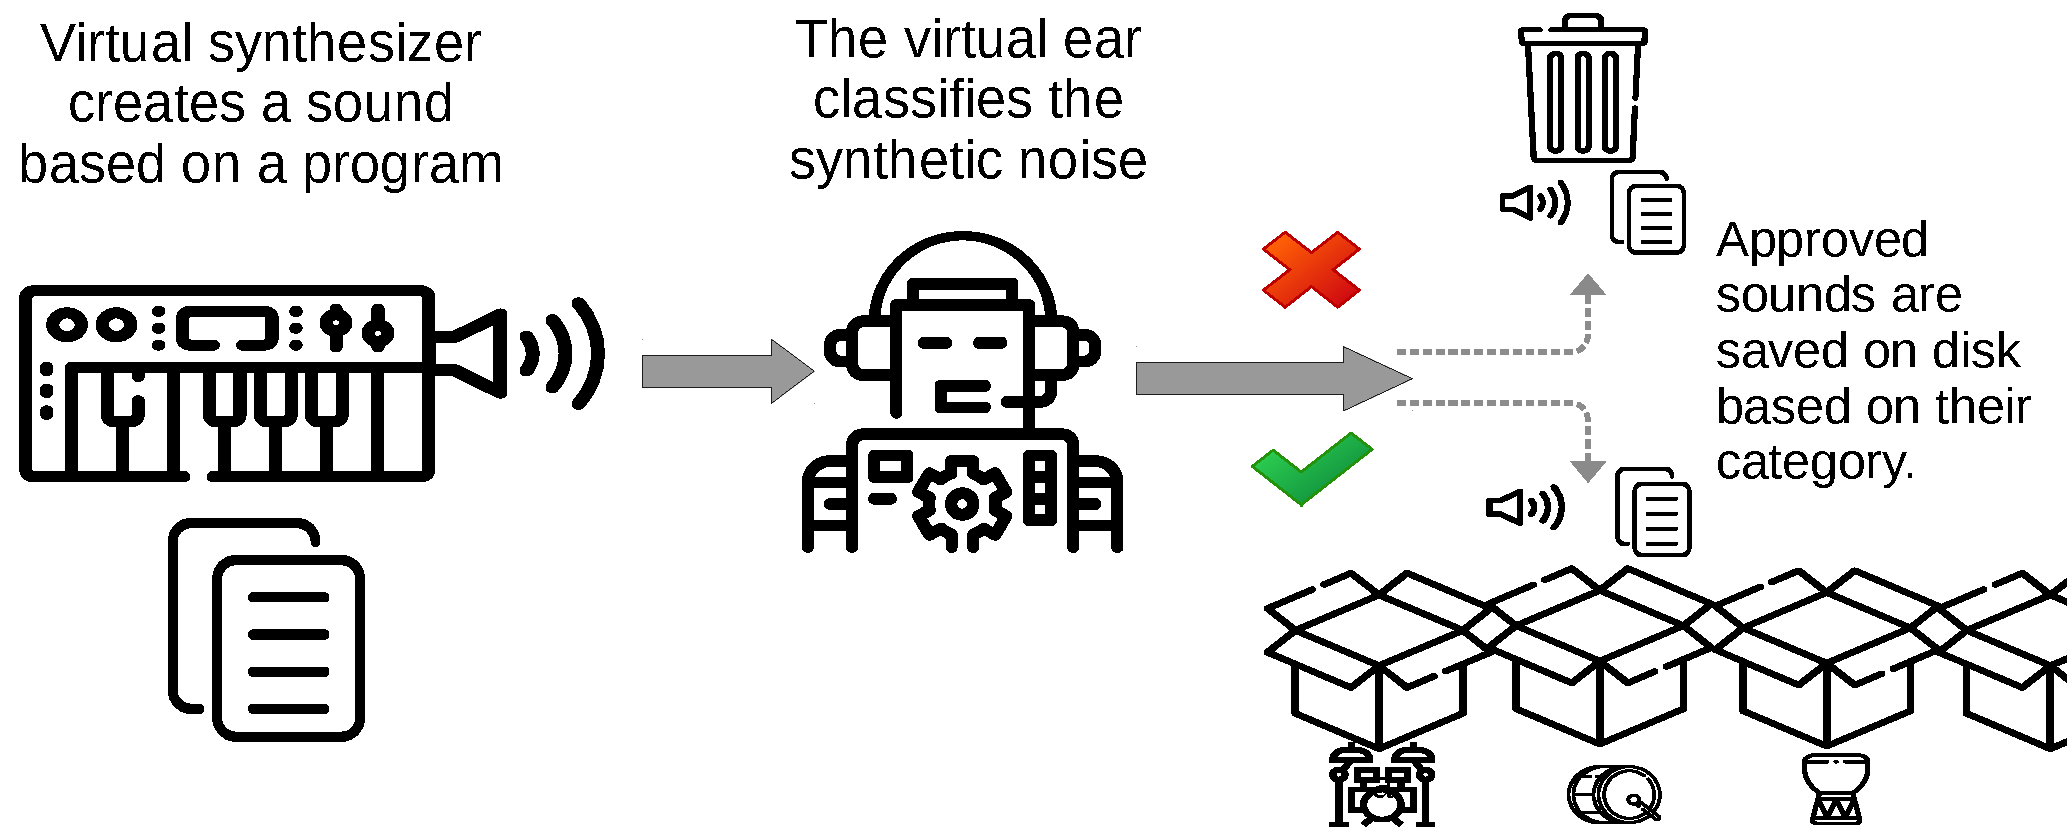
\includegraphics[width=1\linewidth]{images/pipeline.pdf}}}
    \end{center}
    \caption{A blueprint of our desired pipeline which allows each component to be implemented in a number of ways. Our implementations of this pipeline allow for easy parallelization when needed. 
    }
\label{fig:pipeline_outline}
\end{figure}



\subsection{Related Works}
\label{related_works}
\begin{center}
\begin{table}[h]
\resizebox{\linewidth}{!}{\begin{tabular}{|c c c c|} 
\hline
Work & Feature extraction & Synthesis & Specilization & \hline
Oord 2017 & CNN & CNN &Speech& \hline
Yee-King 2018 & LSTM on Paremters & DSP & Synth Pads & \hline
Aouameur 2019 & Latent layer& Decoding of Latent Layers & Percussion & \hline
Ramires 2020 & Latent layer & FeedForward Network & Percussion & \hline
Yamamoto 2020 & GAN & GAN & Speech & \hline
\end{tabular}}
\caption{Quick reference of recent related works}
\end{table}
\label{table:recent_works}
\end{center}
Numerous deep, neural network models have been proposed and utilized for the purpose of signal generation in recent years. WaveGans and WaveNet have been subject to significant improvements and experiments since their proposal~\cite{nsynth2017,yamamoto2020parallel,oord2017parallel}. Particularly relevant are the utilization of variational autoencoders (VAE's) for generation of percussive samples~\cite{aouameur2019neural} and generation of percussive sounds by decoding a small set of latent features~\cite{ramires2020neural}.
Automatic programming of virtual synthesizers has long been a topic of interest. In early 2000s, Interactive Genetic Algorithms (IGA's) were utilized for the generation of new sounds with various sound-engines~\cite{johnson1999exploring,dahlstedt2001creating}. More recent work by Yee-King et al.~\cite{yee2018automatic} used Long short-Term Memory (LSTM) models and genetic algorithms to find the exact parameters used to create a group of sounds. The sounds approximated were made by the same virtual synthesizer, not an external source; making the eventual replication certain even with random search. Since this work appears more focused on pads and textures rather than drums, feature matching appears to not be concerned with the envelope of the sounds but rather the frequency content within arbitrary time windows. Yet another recent work by Esling et al. used a large dataset of over 10,000 presets for a commercial VST synthesizer to learn a latent parameter space which can be sampled for creation of new audio~\cite{esling2019universal}. As stated before, our work explores the rapid approximation of percussion sounds with no previous knowledge about the sonic capabilities of our virtual synthesizer, exploring the actual parameter space rather than its latent representation.

\subsection{Our Approach}
To virtually create novel drum sounds, we need a tractable, generative source of audio; One that deterministically produces audio based on a set of instructions. Additionally, we need a method of evaluation to help us determine which sounds resemble drums and are worth keeping. To enable heuristic search, we would like to know what instructions caused our audio source to make the sounds we liked. Given these two components capable of \textit{generation} and \textit{evaluation} of sounds, we build a generative pipeline of audio as depicted in figure~\ref{fig:pipeline_outline}. The success of this pipeline is dependent on the characteristics of the components responsible for the generation and evaluation of the sounds. We call these two components the \emph{virtual synthesizer} and \emph{virtual ear} respectively.  

\section{Virtual Synthesizer Design}
\begin{table}[htbp]
\centering
\resizebox{\columnwidth}{!}{\begin{tabular}{ |c|c|c| } 
\hline
Parameters & Value Range & notes and constraints\\
\hline \hline
Attack & 0-3 & A-D-S-R values relative\\
Decay & 0-3 & relative to A-S-R\\
Sustain & 0-3 & relative to A-D-R\\
Release & 0-3 & relative to A-D-S\\
OSC type & sine,square,saw & tone type\\
IsNoise & boolean & whether to \newline use OSC type to generate noise\\
Length & 0-1 second & - \\
StartTime & 0-1 second & Length+Start$<$1\\
Amplitude & 0.1-1 & 1 = max amplitude\\
Pitches(notes) & list of pitches &  range of C0(16.35hz) to B9 \\
HP filter Cuttoff & 0-20000hz & -\\
LP filter Cuttoff & 20000-HP & never lower than HP cutoff\\
Filter Order & 4,8,16 & butterworth filter order \\
\hline
\end{tabular}}
\caption{Synthesizer submodule Parameters. Despite the simplicity of the parameters and our efforts at constraining the ranges, the number of parameters that can be randomly chosen for each submodule is in the order of $10^{15}$ }
\label{table:submodule_params}
\end{table}

Sound is product of physical disturbances, causing vibrations in our mediums. Vibrations are perpetuated through air as part of an expanding, spherical front ~\cite{cook1999chap4}. A sound wave can be viewed as the result of a function which governs amplitude through time, where time and amplitude exist in continuous dimensions. Waves can be approximated via a series of samples, associating time steps to a discrete range of amplitude values.~\textit{Digital synthesis} of audio is the process of creating these discrete values.
Unlike the majority of the works mentioned in Section~\ref{related_works}, we do not employ probabilistic models for the synthesizer component. Our decision is based on the following factors:
\begin{itemize}
    \item \textit{Novelty and Creativity}: Given large sets of examples, generative models such as VAEs and GANS have proven capable of generating samples similar to the exemplars. In this work, we are not aiming for perfect imitations; Following Boden's definition of exploratory creativity as an emergent property of generative work within confined rule sets~\cite{boden2009computer}, we work within the limitations of any tractable sound source to create its  approximations of a given sound category. Within the music realm, prominent instance of exploratory creativity is the persistent aesthetics of 8-bit soundtracks, remaining popular long after the original constraints are lifted~\cite{collins2007loop}.
    \item \textit{Interpretability}: Neural networks are often described as black boxes~\cite{basheer2000artificial}. Their highly recursive structure makes modern explanation methods such as saliency maps unreliable~\cite{rudin2019stop}.  
    \item \textit{Speed of Rendering at high sampling rates}: Despite the utilization of powerful GPUs, the standard sampling rate in most audio generation work utilizing neural is under 24 khz \cite{yamamoto2020parallel,oord2017parallel,aouameur2019neural,ramires2020neural}. However, a significant number of untrained human ears can detect a change in quality of audio between sampling rates of 192 khz and the industry standard of 44.1 khz \cite{reiss2016meta}. In this work, we fix our sampling rate to the 48 khz standard. 
\end{itemize}

\begin{figure*}[htbp]
\label{fig_example_sine}
\centering
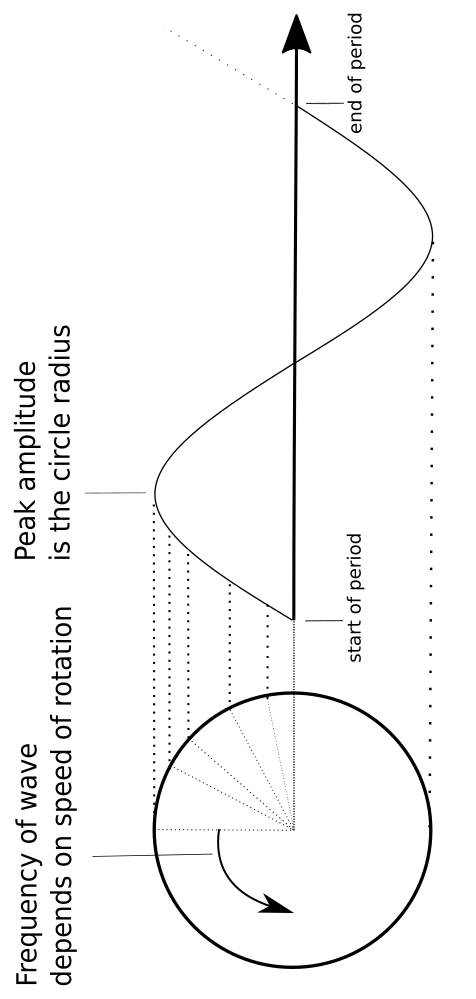
\includegraphics[width=0.45\linewidth,angle =-90 ]{images/periodic_function.png}
\caption{A computer can simulate waveforms by utilizing periodic functions. Digital waveforms are discrete approximations of analogue waves~\cite{mitchell2009basicsynthChap5} }
\end{figure*}

Evaluation of a periodic function such as sine or cosine is the simplest form of software audio generation~\cite{mitchell2009basicsynthChap5}. This generative system is called an \textit{oscillator}. The combination and modification of oscillators are the building blocks of digital signal processing (DSP). Most sounds from the natural environment, and its flora and fauna are more complex than the output of a single oscillator. However, with careful programming, DSP techniques can be used to replicate almost any sound, which is why they have powered coMEMrcial digital synthesizers for over half a century ~\cite{jenkins2019analog}. Another advantage to using DSP for sound generation is that the synthesizers we build using these functions are tractable: the output is determined by the input and reproducible. This makes the evaluation of a set of inputs (or parameters) to our synthesizers  simpler compared to the evaluation of synthesizers that utilize probabilistic models.
 
We opted for a set of classical DSP methods to build our synthesizer. For our project, we used the python based Pippi library for sound generation\footnote{https://github.com/luvsound/pippi}. This library uses a C back-end\footnote{https://github.com/PaulBatchelor/Soundpipe} and focuses on fast offline generation of audio signals. Our virtual synthesizer contains a set of one or more submodules. Each submodule is a self-contained noise making unit. Submodules have identical sets of parameters, but widely different outputs can be achieved depending on the values assigned. The set of parameters available to each submodule is highlighted in Table~\ref{table:submodule_params}. The sonic output of the virtual synthesizer is the normalized addition of the sonic output of its submodules. Our implementation of a synthesizer can have any number of submodules. The parameters that dictate the output signal of each submodule as well as the range of values each parameter can take are shown in table~\ref{table:submodule_params}. We call the number of submodules in each virtual synthesizer the \textit{stack size}. We call the sets of parameter values that characterize a synthesizer's submodules a \textit{program} (analogous to a preset for a VST).  

\section{Virtual Ear}

We are not looking for the perfect imitation of organic drums using a synthesizer. We seek to imitate drums using a synthesizer and even \textbf{prefer} for its generations to retain novel, unusual characteristics. The task assigned to the virtual ear is the rare acceptance of drum-like sounds and the inevitable rejection of most \enquote{noise} outputs from the virtual synthesizer. By definition, we cannot anticipate what these novel drums will sound like. Without manual inspection, all we know is that the accepted sounds are synthesizer noises which the synthetic ear has determined to be similar to drum-sounds. The virtual ear makes two critical decisions: 
\emph{
\begin{quote}
\text{Decision.1 Could the sound be used as a drum?}\label{Decision.1}
\\
\text{Decision.2 If it does sound like a drum, what type of drum should it be?}\label{Decision.2}
\end{quote}
 }
 
\begin{figure}[htbp!]
    \begin{center}
    \textbf{Data Overview}
    \makebox[\textwidth]{
    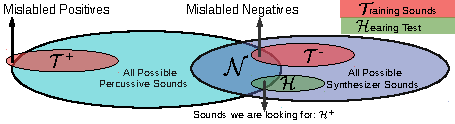
\includegraphics[width=0.95\linewidth]{images/venn_data.pdf}}
    \end{center}
    \caption{ 
    Scales are symbolic (true scales are not measurable and/or subjective).  $\mathcal{N}$ is the set of percussive sounds a synthesizer is capable of making. Our positive samples, $\mathcal{T^{+}}$, is a small fraction of a wide variety of percussive sounds that are conceivable. The size of $\mathcal{T^{-}}$ can be set to any number(we can generate as any number of random samples), but we prefer to keep it no larger than  $\mathcal{T^{+}}$. $\mathcal{H}$ is a series of sounds sent to the ear for classification. The ideal ear will detect  $\mathcal{H^{+}}$, the overlap of $\mathcal{H}$ and $\mathcal{N}$, with high precision and recall. 
    }
\label{fig:ven_data}
\end{figure}
\hypref{Decision.1} requires knowledge of what drums \textbf{do not} sound like, or knowledge of an infinitely large set, which cannot be fully represented via examples. An important consideration is that the source of sounds used in training the model (organic drum sounds) will be fundamentally different from the source of unlabeled sounds we wish to categorize (noise from a synthesizer). This issue is reflective of the OSR problem~\cite{geng2020recent,mundt2019open}. Figure~\ref{fig:ven_data} highlights a number of caveats with this approach. we denote $\mathcal{N}$ as the set of percussive sounds a synthesizer is capable of making. $\mathcal{T^{+}}$, our positive examples, is a set of sound extracted from material drums. $\mathcal{T^{-}}$, is a small subset of an infinite set which is meant to represent all noises which the synthesizer is capable of making. It likely includes sounds in $\mathcal{N}$. could be used as drums. During the hearing test, the virtual ear continually receives synthesizer noises ($\mathcal{H}$) for classification. The performance of the ear is measured by its precision and recall in finding the overlap between $\mathcal{H}$ and $\mathcal{N}$. It is important to ensure that the change in learning domains---particularly with the case of positive examples of percussive instruments---does not interfere with transformation of knowledge from the training of the ear to the hearing test. To maximize the transference of knowledge from one domain to another, we seek to learn from agnostic feature sets that capture fundamental characteristics of the data points.
\subsection{Feature Extraction}
To train our virtual ear, we require generalizable, domain agnostic features. Various works have demonstrated effective reconstruction of signals given their Short-time Fourier Transforms (STFT) ~\cite{nawab1983signal,griffin1984signal}. If the STFT of a signal can be used its reconstruction, perhaps it can be utilized as a source of fundamental features necessary for audible signal categorization. We defined 3 STFT transformation functions which we believe to capture important, unique attributes of percussive sounds (figure ~\ref{fig:stackspectrums}). Our transformations are GPU based, allowing their application in tandem to the training of the classifier or tuning of STFT transformation during hyper-paramter optimization (see Section~\ref{---}).

\subsection{Ear Types}
\label{classifiers}
Two groups of classifiers are implemented: \emph{two phased ears} (TPEs) and \emph{Mixed Ear Models} (MEMs). TPEs combine different models specializing in ~\hypref{Decision.2} or ~\hypref{Decision.1} and trained only with our transformation functions. MEMs are a proof of concept attempt at addressing the OSR problem by usage of autoencoded representation of sounds as features. MEMs are trained using highly compressed, automatically encoded representation of sounds and can give simultaneous answers to both questions. Model specifications for TPE and MEMs can be found in Appendix~\ref{appendix:C}. We speculate that the features used to represent sounds plays a much more important role in determining outcomes, particularly when working with relatively small datasets. 

The features used by MEMs are encodings extracted from the latent layer of an autoencoder trained with MixedDB. To better understand the delineation potential of the encoded features, 64-dimensional latent representation of 20\% of MixedDB and 1000 Noise sounds were projected onto a 2 or 3-dimensional planes using t-SNE. Referring to~\hypref{Decision.1} and~\hypref{Decision.2}, we expect the drum sounds to be clustered together, with the majority of the synthetic noise sounds appearing away from these clusters. The projections confirmed that this is the case(see Appendix~\ref{appendix:E}). We are most interested in synthetic noise sounds which appear within or near these clusters. Do these synthetic noise sounds have drum like characteristics?\\ 
To test this, we implemented interactive projection graphs. These graphs allow interactions such as playing the samples(by hovering the cursor on-top) and movement of the scene camera. Manual inspections revealed a noticeable, positive correlation between distance and similarity of a synthetic sound to drum clusters.

\section{Pipelines and Surveys}
\label{gens}
\label{surveys}
With our virtual synthesizer and virtual ears in place, we build two pipelines, one using all TPE models and the other using our best MEM model. To assess the performance of each pipeline, we randomly create drum programs and generate and the corresponding signal. This signal is then fed through the ear model to determine if the signal is percussive. If so, a category is assigned to the sound. This sound and the corresponding synthesizer program are saved to hard-disk. Here we assess the success rate of two different pipelines by manual inspection of sounds it has categorized as drums, as well as the category of those drums. The authors of this work attempt their own categorization of a randomly selected subset of each pipeline's results. We cross reference the manual categorizations with the categories assigned by the virtual ear: Do we agree that the sounds are percussive? Do we agree with the drum group assigned to the percussive sounds?
 
 \section{Survey of Two-Phased Ear Performance}
   
\begin{table}[htbp]
 \resizebox{\linewidth}{!}{\begin{tabular}{||c c c c c c c||} 
 \hline
 Drop Rule & Size & HvH & H+FC & H+CNN & H+ALL & 3 models \\ [0.5ex] 
 \hline
 No Drops & 257 &0.37 & 0.35 & 0.36 & 0.36 & 0.28\\ 
 \hline
 Assigned \enquote{Bad} By Both & 236 & 0.31 & 0.37 & 0.37 & 0.38 & 0.30 \\
 \hline
 Assigned \enquote{Bad} By Either & 180 & 0.47 & 0.50 & 0.48 & 0.48 &  0.34 \\
 \hline
 Assigned \enquote{Bad} or \enquote{Other} By Either & 154 & 0.47 & 0.59 & 0.54 & 0.50 &  0.35 \\
 \hline
\end{tabular}}
\caption{\label{kappa_table_TPE}Table of Fleiss' kappa coefficient to measure the degree of agreement between persons (HvH), persons with FC model (H+FC), persons with CNNLSTM model, persons with all models (H+ALL), and between the 3 models. \enquote{Drop Rule} column indicates if any samples were dropped. We show the measurements after dropping samples if they are deemed bad by either or both responders. We also show measurements after dropping the \enquote{other} category along with samples deemed bad by either responder. }
\end{table}
To measure the quality of the samples produced by our pipeline combined with the TP ear models, we run the model until an adequate number of samples in each category are saved to disk. Next, we randomly generated around 50 samples in the following categories: \enquote{snare}, \enquote{kick}, \enquote{hat}, \enquote{clap} and \enquote{other} (combination of rims, 
shakers and unusual percussive sounds). This gave us a total of 257 samples. These samples were determined to be percussive and then categorized by 4 different models (FC, CNNLSTM, E+F and AVG). We ensured a balanced division between samples of stack size 1, 2 and 4 (each stack is responsible for a third of the samples under each category). Both reviewers then categorized these samples without knowledge of other categorizations (person or computation models). Additionally, each responder had the option of labeling samples as \enquote{bad} for samples that they deemed not percussive. 

We assess the reliability of agreement between persons and categorization models via the Fleiss' kappa coefficient \cite{fleiss1971measuring}. The value of 0 or less for this coefficient indicates no agreement beyond random chance, and the value of 1 indicating perfect agreement. Our kappa measurements showcased in~\ref{kappa_table_TPE} lie within the 0.35-0.45 range, indicating mild to moderate agreement between persons and machines. We again measure this coefficient after dropping samples that were categorized as \enquote{bad} by the authors, as samples that persons deem to be \enquote{bad} indicate a failure in Phase 1 and should not have been categorized by the models at all.

\section{Survey of Mixed-Models Ear Performance}
 Keeping the other components of the pipeline the same, we replace the two-phased ear in the previous pipeline with the MME. Our survey differs from the previous survey in that the pipeline only creates the four drum categories. Our main concern here is changes in the amount of \enquote{bad} samples. We show measurements before and after dropping all \enquote{bad} and \enquote{other} samples for a fairer comparison with the TPE pipeline.

 \begin{table}[t]
 \resizebox{\linewidth}{!}{\begin{tabular}{||c c c c||} 
 \hline
 Drop Rule & Size & HvH & H+MME \\
 \hline
 No Drop & 300 & 0.336 & 0.250\\ 
 \hline
 Assigned Bad By Both & 249 & 0.200 & 0.260 \\
 \hline
 Assigned Bad By Either & 151 & 0.460 &  0.473 \\
 \hline
Assigned \enquote{Bad} or \enquote{Other} By Either  & 120 & 0.620   &  0.587 \\
 \hline
\end{tabular}}
\caption{\label{kappa_table_MME}Table of Fleiss' kappa coefficient to measure the degree of agreement between persons (HvH) and persons and MME. We also measure the agreeability scores after dropping bad samples if both or either persons assigned the sample as such. We also measure agree-ability when all samples deemed \enquote{bad} or \enquote{other} by either person are removed.}
\end{table}

\subsection{Takeaways from These Surveys}
\label{survey2_takeaway}
The results from the two surveys are not easily comparable. However, no major improvements in agree-ability or a decrease in the number of bad samples can be seen, in fact, the opposite is more likely to be true. However, we are yielding comparable results to the TPE pipeline despite having a fraction of the features to learn from (latent layer + 10 envelope features). This shows that latent layers of an autoencoder network can be used as a low-dimensional proxy for representation of more complex inputs, despite the autoencoder not being trained for such a task. Agree-ability scores for MME pipeline are often lower, but we reiterate that this can be caused by having two out of six (rather than one out of six in the TPE pipeline) categories which are exclusive to survey responders. Supporting this hypothesis is the notable improvement in agree-ability observed after dropping all \enquote{bad} and \enquote{other} samples. Here, both persons agree with each other and with the MME at a stronger rate than in the TPE pipeline, despite having similar number of samples (120 for MME and 154 for TPE) and equal number of categories to choose from. This values are observed in the last rows of tables~\ref{kappa_table_TPE} and ~\ref{kappa_table_MME}. The higher DVD categorization accuracy achieved by the mixed-model ear compared to the best two-phaased ear is consistent with this observation: Given that the sound being categorized is a drum, the MME will yield better results that the TPE. However, the MME pipeline does not yield better results in the DVN task. 
\begin{itemize}
    \item The survey brings into question the reliability of our phase 1 models, as 30\% of the generated samples were deemed not percussive by at least 1 reviewer and 8\% by both reviewers
    \item The task of categorizing synthetic drums is difficult. Survey shows that the scale of agreement within persons as well as between persons and various model combinations is moderate at best, even after removal of \enquote{bad} samples.  While the same models can easily achieve 98+ percent accuracy when tested on sounds from physical drum samples. 
    \item While there is much room for improvement, our pipelines can generate and categorize drums and percussive sounds with a promising degree of success. 
\end{itemize}
\bibliographystyle{apacite}
\bibliography{CSMC_MUME_LaTeX_Template.bib}

\begin{appendices}
\chapter{Datasets}
\label{appendix:A}
\begin{table}[h!]
\centering
\begin{tabular}[width=\paperwidth]{|l|l|l|l|l|l|l|l|l|l|}
\hline
DB Name & kick & snare & clap & tom\_high & tom\_mid & tom\_low & hihat\_closed &  hihat\_open & rim \\ \hline
MixedDB & 648 & 732 & 118 & 179 & 139 &  188 & 187 & 280 & 105 \\\hline
\end{tabular}
\caption{Database 1: Mixed sources}
\label{db:self}
\end{table}

\begin{table}[h!]
\centering
\begin{tabular}{|l|l|l|l|l|l|l|l|l|}
\hline
DB Name & kick & snare & clap & tom & clap & hat & rim & shaker  \\ \hline
RadarDB & 1054 & 842   & 353 & 349 &  353 & 1561& 131 & 121 \\ \hline
\end{tabular}
\caption{Database 2: Royalty free sounds sourced from \enquote{Music Radar}}
\label{db:radar}
\end{table}

\begin{table}[h!]
\centering
\begin{tabular}{|l|l|l|l|l|l|}
\hline
 DB Name & kick & snare & clap & hat & other \\\hline
 FreeDB & 533 & 372 & 230 & 105 & 281 \\ \hline
\end{tabular}
\caption{Database 3: Free sounds sourced from the \enquote{Sample Swap} project. Simplified for our purposes. The version available for download contains more sample groups. The \enquote{other} category contains a variety of percussive sounds.}
\label{db:sampleswap}
\end{table}


\begin{table}[h!]
\centering
\begin{tabular}{|l|l|l|l|}
\hline
 Synth Noise Type & 1 Stack & 3 Stacks  & 5 Stacks \\ \hline
 Number of Examples & 2000 & 2000 & 2000 \\ \hline
\end{tabular}
\caption{Database of random noise examples from our virtual synthesizers}
\label{db:noise}
\end{table}

%=============
\chapter{Audio Transformation Functions}
\label{appendix:B}
\begin{figure}
\centering
\textbf{Visual Representation of Raw Features}\par\medskip
    \subcaptionbox{Recorded hat sample}{    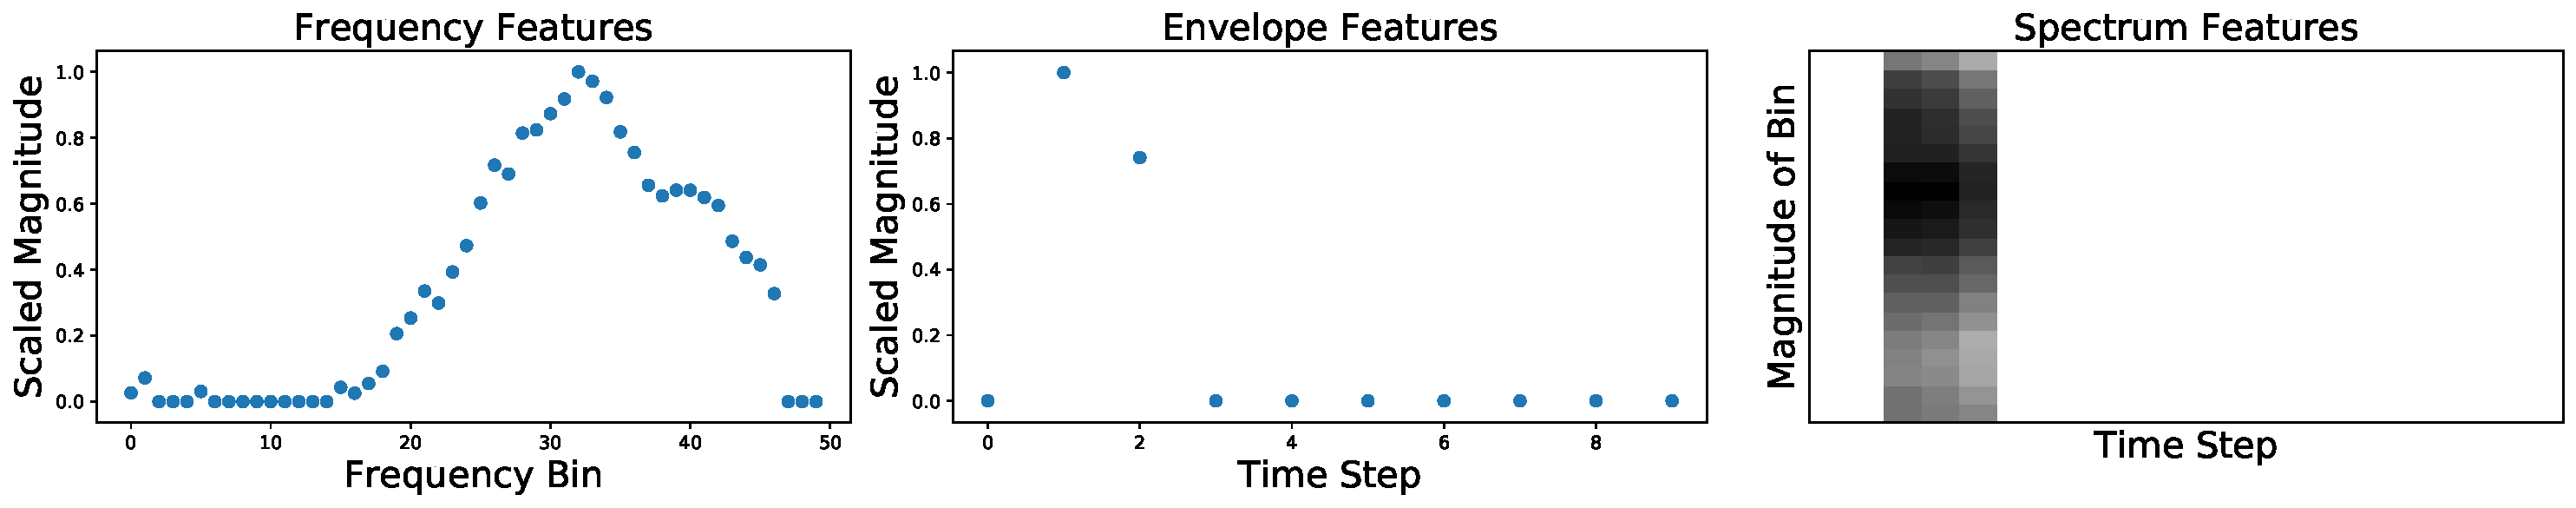
\includegraphics[width=1\columnwidth]{images/ff1.pdf}
    }
    \subcaptionbox{Randomly generated audio with percussive qualities, resembling a tight snare}{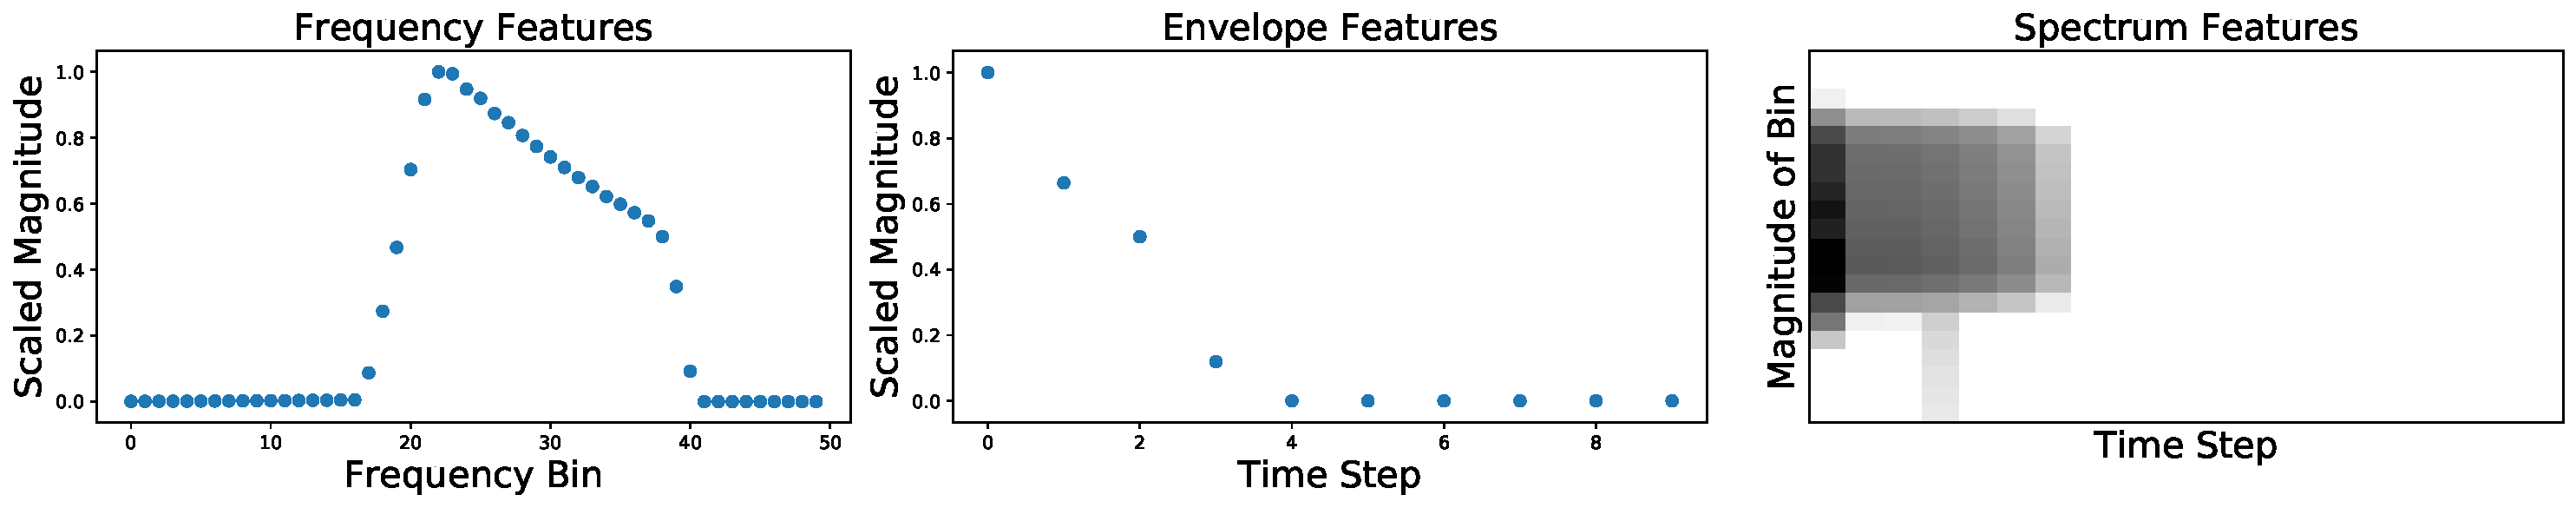
\includegraphics[width=1\columnwidth]{images/ff2.pdf}}
    \subcaptionbox{A randomly generated noise with a percussive envelop but non-percussive frequency features (modulated pitch)}
    { 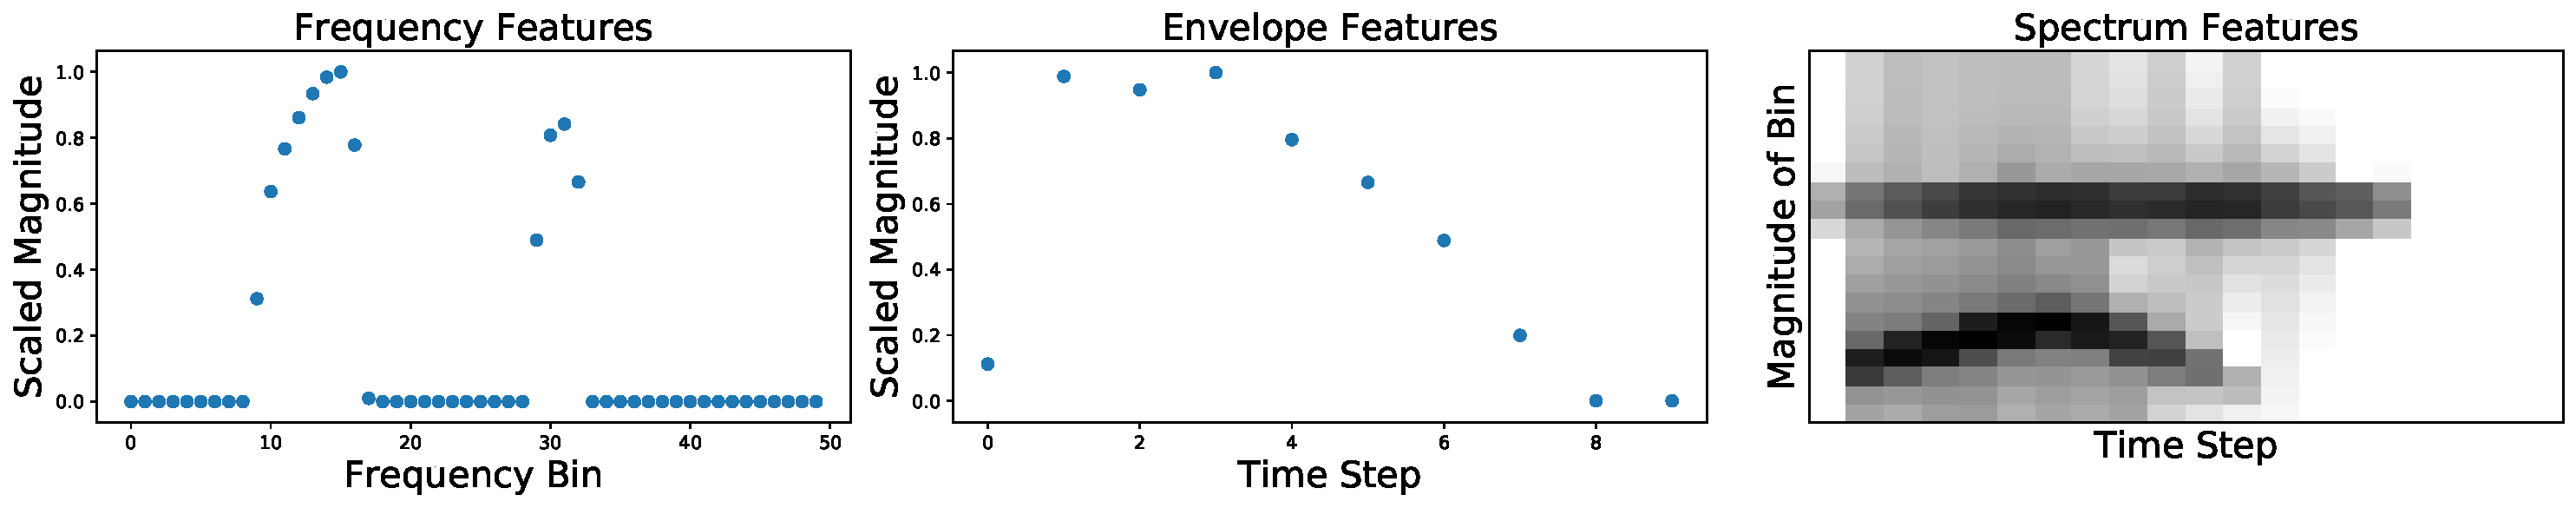
\includegraphics[width=1\columnwidth]{images/ff3.pdf}}
\caption{Graphed representation of features extracted for 3 different samples. Sample $a$ is a recorded hat from our database. sample $b$ is an example of randomly generated noise with percussive qualities that we found suitably similar to a snare sound. Sample $c$ is an example of a randomly generated noise where the spectrum features are necessary for proper classification.}
\label{fig:stackspectrums}
\end{figure}
\begin{enumerate}
\item Envelope Transformation: Represents changes in loudness for the duration of the signal. Using STFT we generate a matrix $M_{i \times j}$ with rows $i$ and columns $j$ corresponding to time steps and frequency bins respectively. Values $v_{i \times j}$ indicating the magnitude of the frequency bin $j$ at each time-step $i$. Information about the envelope of the signal can be extracted by summing the values of $M$ for each time-step (or row $i$), giving us a feature vector that is normalized to the range of 0 to 1. The information contained in this vector is an alternative to Root-Mean-Square measurements of a sliding window over the signal.
\item Frequency Transformation: A static, normalized snap-shot of the the frequencies present within the audio. The calculation of this feature vector is similar to the envelope, but the summation is done along the frequency axis. Another important distinction is that since capturing an adequate frequency resolution is important for this transformation, we utilized shorter hop-sizes and wider windows. A Mel Scale transformation was also applied in hopes that the captured features better represent human perception of frequencies. 
\item Spectrum Transformation: This function is simply a Mel Scaled STFT with its values normalized from 0-1. Spectrograms contain more information about the original signal but their analysis requires more complex computational methods.
\end{enumerate}

%================
\chapter{Virtual Ear Classifier Definitions}
\label{appendix:C}
\section{Two Phased models}
Using the described features, we trained several neural network models for Phase 1 and 2 in the Pytorch environment. The task of Phase 1 is to separate drums from not-drums (DrumVsNotDrum, or DVN). The task of Phase 2 is to categorize drums and percussion (DrumVsDrum, or DVD). We kept our feature space small, making it viable for feature selection and model design to be done on a trial and error basis. For all models, accuracy is calculated by prediction of all test dataset labels and the loss function and optimizer are Categorical-CrossEntropy and Adam respectively. Training continues until no reduction in loss and accuracy is observed in 10 epochs.  All activation functions are PReLU:
\begin {enumerate}
\item FC-DVN: Fully connected network trained on Envelope features, reaching 97\% accuracy on our test data for Phase 1. With size of 10x5x10.
\item CNNLSTM-DVN: A combination of CNN and LSTM models, where the CNN model extracts higher level features that are fed temporally to an LSTM cell. This model is trained on spectrum data and reaches 98\% accuracy on our test set. Its structure is the combination of a CNN with 2 output channels and kernel size $(7,3)$; Followed by an LSTM model of hidden size 800 and a fully connected layer of size 20x2.
\item E+F-DVD: A fully connected model trained on a concatenation of envelope and frequency features. Reaching 80\% accuracy for 6-way drum categorization in Phase 2. Size of 50x10x2x6.
\item CNN-DVD: A CNN model trained on Spectrum features. Reaching 82\% accuracy in a 6-way drum categorization in Phase 2. A combination of a CNN model with output channel size of 4, kernel of size of 5, another CNN model with output channel size of 8 and kernel of size 3. Followed by a fully connected network of shape 100x20x6.
\item FC-DVD: Fully connected 3 layer neural net with 78\% accuracy for 6-way drum categorization in Phase 2. Size of 400x200x50.
\end{enumerate}
Unlike EE models, parameters are hand-picked and un-tuned. Higher accuracy rates in these models do not necessarily translate to higher agreeableness with surveyors. Since the positive sounds in the hearing test are sourced from a synthesizer, model accuracy on test data alone cannot be relied upon when the domain of sounds 
being categorized is switched.

\chapter{AutoEncoder Structures and Hyper-Parameter Optimization}
\label{appendix:D}
\section{Possible Model Structures}
\begin{table}[[h]
\begin{tabular}{|p{28mm}|p{25mm}|p{23mm}|p{50mm}|}
\hline
Layer-\# & Out Shape & Param Num & Details  \\ \hline
Conv2d-1 & [-1, 8, 30, 20] &   208 & Encoder's input \newline
Num. Channels:8\newline
kernel:5x5\newline                  
stride:1\newline    
padding:2 \\ \hline
ReLU-2 & [-1, 8, 30, 20] &   0 & \\  \hline
MaxPool2d-3 & [-1, 8, 15, 10] & 0 &  kernel:5x5 \newline
stride:2 \\ \hline
Dropout-4 & [-1, 8, 15, 10] & 0 &  \\ \hline
Linear-5 & [-1, 8] & 9,608 & Encoder's output \\ \hline
Linear-6 & [-1, 256] & 2,304 & Decoder's Input \\ \hline
Dropout-7 & [-1, 256] & 0 &  \\ \hline
Linear-8 & [-1, 600 ] &  154,200& Decoder's output\\ \hline
\end{tabular}
\caption{CNN model design with latent size of 8. 30 and 20 are the assumed frequency bins and step size. Total number of parameters is 166,320. }
\label{table:CNNAUTOENCODER}
\end{table}

\begin{table}[[h]
\begin{tabular}{|p{28mm}|p{25mm}|p{23mm}|p{50mm}|}
\hline
Layer-\# & Out Shape & Param Num & Details  \\ \hline
Linear-1 & [-1, 128]  & 76,928 & Encoder's input \\ \hline
Dropout-2 & [-1, 128] & 0 &  \\ \hline
Linear-3 & [-1, 8] & 9,608 & Encoder's output \\ \hline
Linear-4 & [-1, 128] & 2,304 & Decoder's Input \\ \hline
Dropout-5 & [-1, 128]  & 0 &  \\ \hline
Linear-6  & [-1, 600 ] &  77,400 &Decoder's output\\ \hline
\end{tabular}
\caption{Fully connected model with only 1 hidden dimension for encoder and decoder. Designed assumes latent size of 8. 30 and 20 are the assumed frequency-bins and step-size values. Total number of parameters is 156,512.}
\label{table:FC1_AUTOENCODER}
\end{table}

\begin{table}[[h]

\begin{tabular}{|p{28mm}|p{25mm}|p{23mm}|p{50mm}|}
\hline
Layer-\# & Out Shape & Param Num & Details  \\ \hline
Linear-1 & [-1, 128]  & 76,928 & Encoder's input \\ \hline
Dropout-2 & [-1, 128] & 0 &  \\ \hline
Linear-3 & [-1, 32]  & 4,128 & \\ \hline
Dropout-4 & [-1, 128] & 0 &  \\ \hline
Linear-5 & [-1, 8] & 9,608 & Encoder's output \\ \hline
Linear-4 & [-1, 32] & 2,304 & Decoder's Input \\ \hline
Dropout-5 & [-1, 32]  & 0 &  \\ \hline
Linear-4 & [-1, 128] & 2,304 & \\ \hline
Dropout-5 & [-1, 128]  & 0 &  \\ \hline
Linear-6  & [-1, 600 ] &  77,400 &Decoder's output\\ \hline
\end{tabular}
\caption{Fully connected model with 2 hidden dimensions for encoder and decoder. Designed assumes latent size of 8. 30 and 20 are the assumed frequency-bins and step-size values. Total number of parameters is 163,232.}
\label{table:FC2_AUTOENCODER}
\end{table}
\begin{table}[htbp!]
\centering
\begin{tabular}{|p{6cm}|p{6cm}|}
\hline
Hyper-Param. & Value  \\ \hline
Model Type      &  CNN  \\ \hline
Optimizer       & Adam  \\ \hline
Hidden Layers   & -  \\\hline
Learning Rate   &  0.001145\\ \hline
Frequency Bins & 30 \\ \hline
Time Steps & 20 \\ \hline
Latent Size & 64 \\ \hline
Regularization & 3.25^{-6}\\ \hline
Dropout Rate & 0.5 \\ \hline
\end{tabular}
\caption{Top performing hyper-parameter set}
\label{table:best_params}
\end{table}
\chapter{Embedded Feature Visualization}
\label{appendix:E}
\begin{figure}[]
\centering
\textbf{2 Dimensional Projection of Latent Variables}\par\medskip
 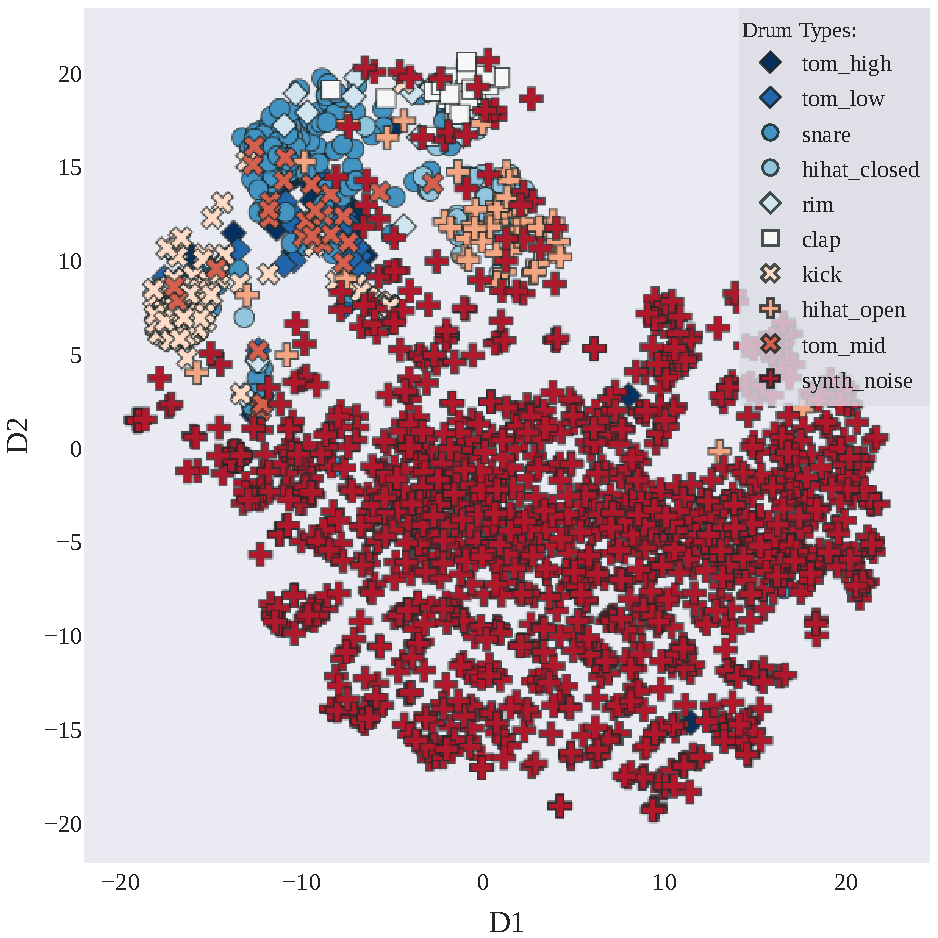
\includegraphics[width=0.90\linewidth]{images/t-SNE_2d.pdf}
\caption{Projection of an embedding model's low dimensional encoding on to a 2D plane. We implemented interactions for these graphs for manual inspection of samples. }
\label{fig:2d_tsne}
\end{figure}

\begin{figure}[]
\centering
\textbf{3D t-SNE Projection}\par\medskip
\mbox{\subfloat[]{\label{subfig:1} \fbox{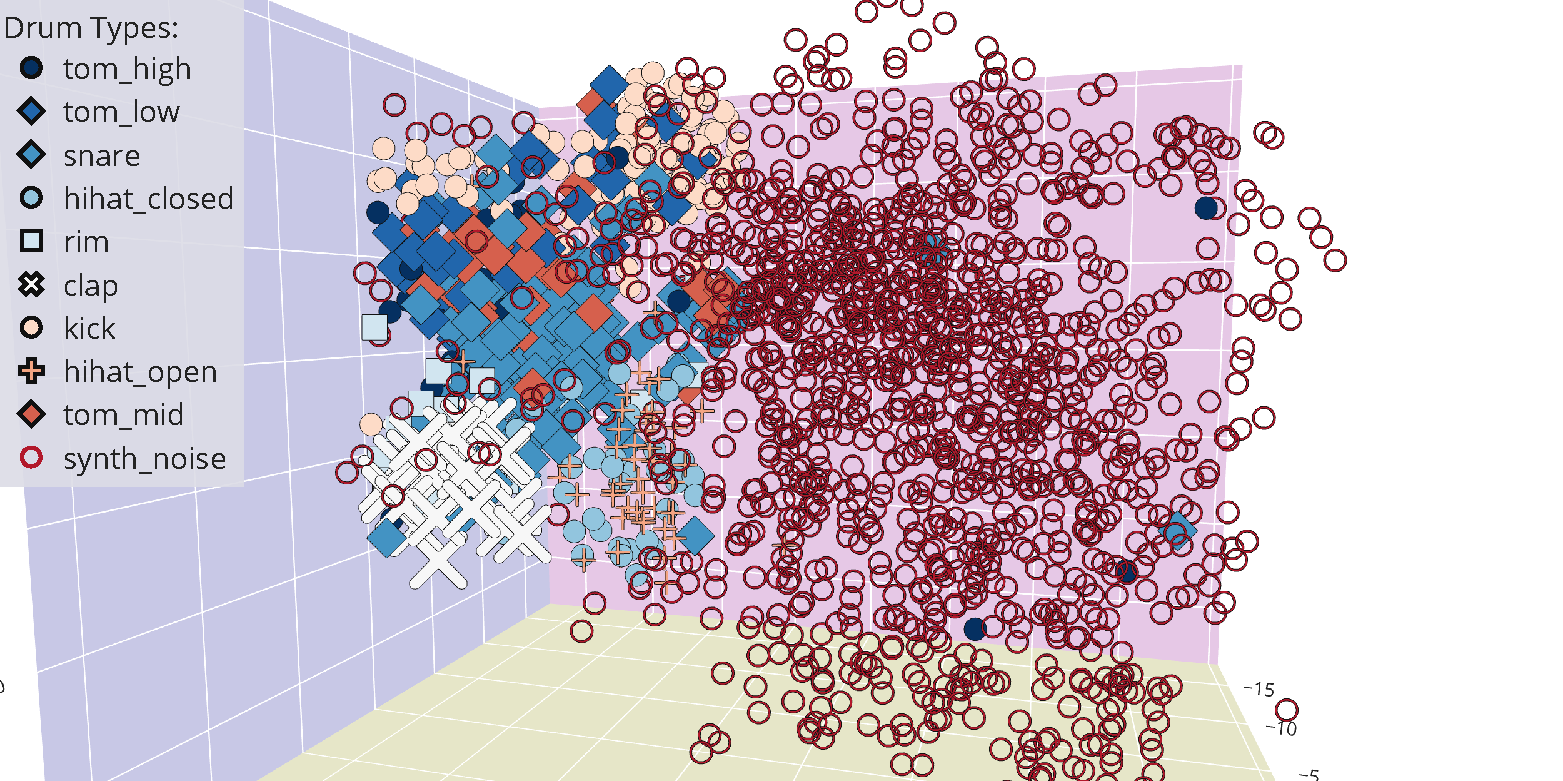
\includegraphics[width=12cm,height=6.8cm]{images/3d_t-SNE_symdrum_type_cam0.pdf}}}}

\mbox{\subfloat[]{\label{subfig:2} \fbox{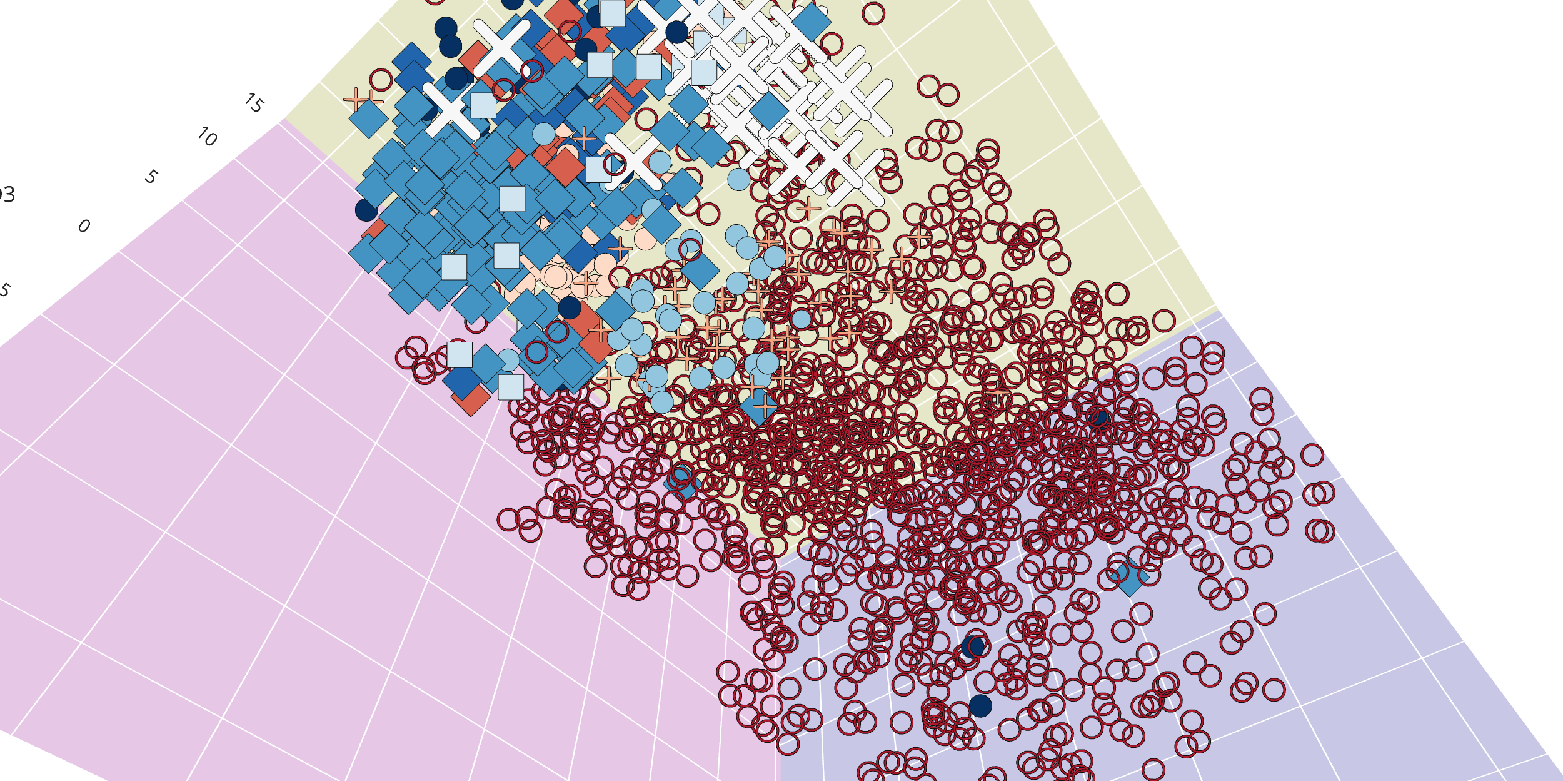
\includegraphics[width=12cm,height=6.8cm]{images/3d_t-SNE_symdrum_type_cam3.pdf}}}}

\fbox{\mbox{\subfloat[]{\label{subfig:2} 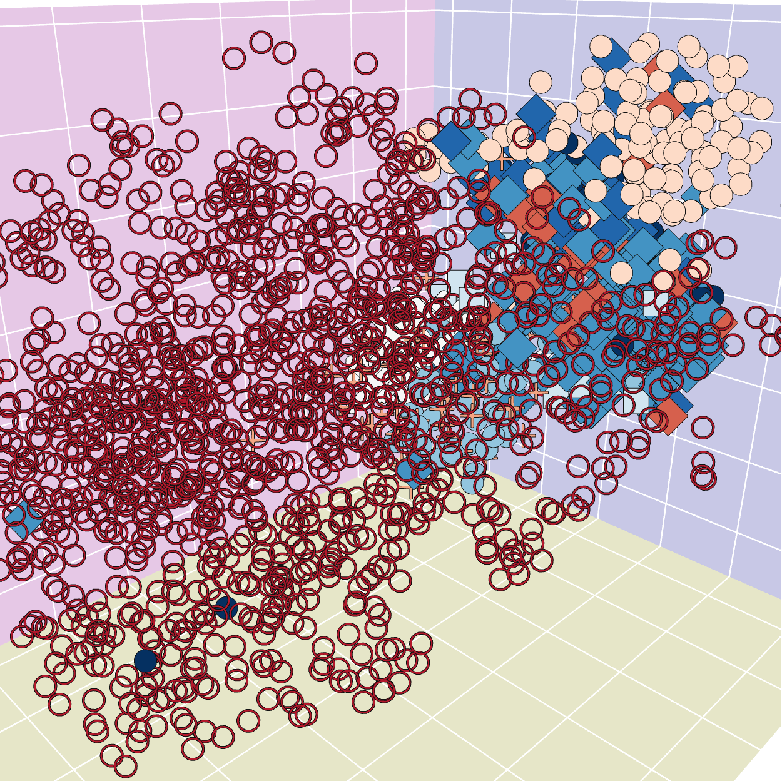
\includegraphics[width=6cm,height=6cm]{images/3d_t-SNE_symdrum_type_cam1.pdf}}}
\mbox{\subfloat[]{\label{subfig:2} 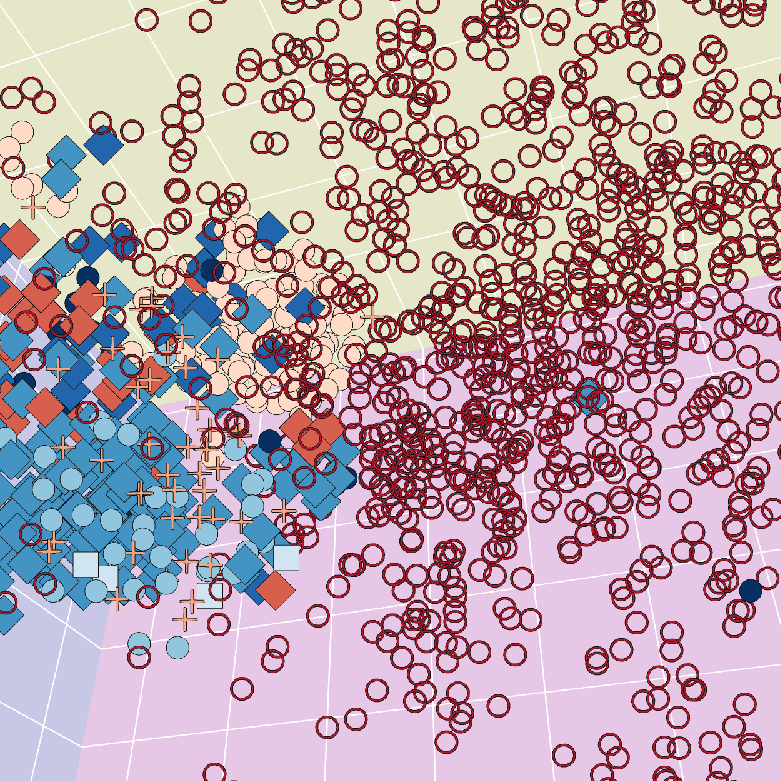
\includegraphics[width=6cm,height=6cm]{images/3d_t-SNE_symdrum_type_cam2.pdf}}}}
\caption{3D projections of the data used for Figure~\ref{fig:2d_tsne}. Interactive demos are also implemented for 3D projections.}
\label{fig:3d_tsne}
\end{figure}


\end{appendices}
\end{document}
